%=====================================================
\section{Maximum, Minimum, Chain and Antichain}
%=====================================================

%-----------------------------------------------------
\begin{frame}{Maximum and Minimum Elements}

\textbf{Let } $(P,\leq)$ \textbf{ be a partially ordered set.}

\vspace{0.5cm}

\begin{block}{Maximum Element}

\vspace{0.1cm}

An element $m\in P$ is called the \textbf{maximum (greatest)} element if

\[
\forall x\in P,\; x\leq m.
\]

\end{block}

\vspace{0.4cm}

\begin{block}{Minimum Element}

\vspace{0.1cm}

An element $n\in P$ is called the \textbf{minimum (least)} element if

\[
\forall x\in P,\; n\leq x.
\]

\end{block}

\end{frame}

%-----------------------------------------------------

\begin{frame}{Example using a Hasse Diagram}

\centering

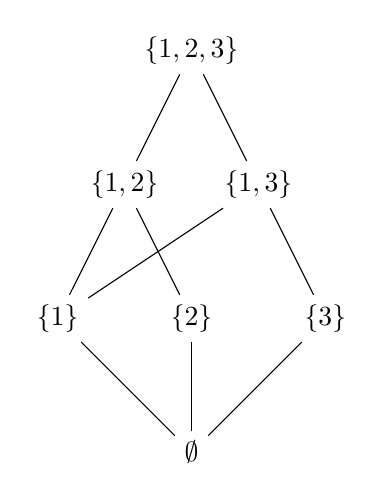
\begin{tikzpicture}[scale=0.85]

\node (a) at (0,0) {$\emptyset$};

\node (b) at (-2,2) {$\{1\}$};
\node (c) at (0,2) {$\{2\}$};
\node (d) at (2,2) {$\{3\}$};

\node (e) at (-1,4) {$\{1,2\}$};
\node (f) at (1,4) {$\{1,3\}$};

\node (g) at (0,6) {$\{1,2,3\}$};

\draw (a)--(b);
\draw (a)--(c);
\draw (a)--(d);

\draw (b)--(e);
\draw (b)--(f);

\draw (c)--(e);

\draw (d)--(f);

\draw (e)--(g);
\draw (f)--(g);

\end{tikzpicture}
\[
\boxed{
\begin{aligned}
\text{Minimum Element} &= \emptyset\\
\text{Maximum Element} &= \{1,2,3\}
\end{aligned}
}
\]

\end{frame}

%-----------------------------------------------------

\begin{frame}{Chain and Antichain}

\begin{block}{Chain}

A \textbf{chain} is a subset of a poset in which every pair of
elements is comparable.
\[
\forall a,b\in C,\;
a\leq b
\;\text{or}\;
b\leq a.
\]
Example:
\[
\emptyset
\subseteq
\{1\}
\subseteq
\{1,2\}
\subseteq
\{1,2,3\}
\]

\end{block}

\begin{block}{Antichain}

An \textbf{antichain} is a subset in which no two distinct
elements are comparable.
\[
\forall a\neq b,\;
a\nleq b
\land
b\nleq a.
\]
Example: 
\[
\{\{1\},\{2\},\{3\}\}
\]

\end{block}

\end{frame}